\documentclass[a4paper]{article}
%%%%%%%%%%%%%%%%%%%%%%%%%%%%%%%%%%%%%%%%%%%%%%%%%%%%%%%%%%%%%%%%%%%%%%%%%%%%%%%%%%%%%%%%
 
%    Eric Lee's LaTeX Preamble
%    Primarily for Problem Sets and Beamer Presentations
%    Email: ericlovesmath@gmail.com
%    Github: https://github.com/ericlovesmath
%    Much thanks to Gilles Castel (https://castel.dev/)
 
%%%%%%%%%%%%%%%%%%%%%%%%%%%%%%%%%%%%%%%%%%%%%%%%%%%%%%%%%%%%%%%%%%%%%%%%%%%%%%%%%%%%%%%%

% Basic Packages
\usepackage[utf8]{inputenc}
\usepackage[T1]{fontenc}
\usepackage[margin=1in,footskip=0.25in]{geometry}
\usepackage{textcomp}
\usepackage{graphicx}
\usepackage{subcaption}
\usepackage{booktabs}
\usepackage{float}
\usepackage{multicol}
\usepackage{emptypage}
\usepackage{import}
\usepackage{pdfpages}
\usepackage{transparent}
\usepackage{hyperref}
\usepackage{url}
\hypersetup{
    colorlinks,
    linkcolor={black},
    citecolor={black},
    urlcolor={blue!80!black}
}
\usepackage[dvipsnames]{xcolor}
\usepackage[inline]{enumitem}

% Math Mode Packages
\usepackage{amsmath, amsfonts, mathtools, amsthm, amssymb}
\usepackage{mathrsfs}
\usepackage{cancel}
\usepackage{siunitx}

% Fix Parskip bug with Amsthm (removes gap before theorem envs)
% https://tex.stackexchange.com/questions/450551/theorems-and-parskip
\usepackage{parskip}
\usepackage{etoolbox}
\makeatletter
\patchcmd\deferred@thm@head
  {\addvspace{-\parskip}}
  {}
  {}{\typeout{\string\deferred@thm@head patch failed!}}
\makeatother 


% TikZ and Plotting
\usepackage{tikz}
\usepackage{tikz-cd}
\usepackage{pgfplots}
\usetikzlibrary{intersections, angles, quotes, calc, positioning}
\usetikzlibrary{arrows.meta}
\tikzset{ force/.style={thick, {Circle[length=2pt]}-stealth, shorten <=-1pt} }
\pgfplotsset{compat=1.13}

% Code Formatting
\usepackage{listings}
\definecolor{codegreen}{rgb}{0.0, 0.6, 0.0}
\definecolor{codegray}{rgb}{0.5, 0.5, 0.5}
\definecolor{codepurple}{rgb}{0.58, 0.0, 0.82}
\definecolor{backcolour}{rgb}{1.0, 1.0, 1.0}
% \definecolor{backcolour}{rgb}{0.95, 0.95, 0.92}
\lstdefinestyle{mystyle}{
    backgroundcolor=\color{backcolour},
    commentstyle=\color{codegray},
    keywordstyle=\color{magenta},
    numberstyle=\tiny\color{codepurple},
    stringstyle=\color{codegreen},
    basicstyle=\ttfamily\footnotesize,
    breakatwhitespace=false,
    breaklines=true,
    captionpos=b,
    keepspaces=true,
    numbers=none,
    numbersep=5pt,
    showspaces=false,
    showstringspaces=false,
    showtabs=false,
    tabsize=2
}
\lstset{style=mystyle}

% Misc
\pdfminorversion=7
\pdfsuppresswarningpagegroup=1

%%%%%%%%%%%%%%%%%%%%%%%%%%%%%%%%%%%%%%%%%%%%%%%%%%%%%%%%%%%%%%%%%%%%%%%%%%%%%%%%%%%%%%%%

% Math Mode Mappings
\newcommand\N{\ensuremath{\mathbb{N}}}
\newcommand\R{\ensuremath{\mathbb{R}}}
\newcommand\Z{\ensuremath{\mathbb{Z}}}
\newcommand\Q{\ensuremath{\mathbb{Q}}}
\newcommand\C{\ensuremath{\mathbb{C}}}
\renewcommand\O{\ensuremath{\emptyset}}
\let\implies\Rightarrow
\let\impliedby\Leftarrow
\let\iff\Leftrightarrow
\let\epsilon\varepsilon

\newcommand{\op}[1]{\left\|#1\right\|_\text{op}}
\newcommand{\E}{\operatorname{\mathbb{E}}}
\newcommand{\Var}{\operatorname{Var}}
\newcommand{\Bias}{\operatorname{Bias}}
\newcommand{\MSE}{\operatorname{MSE}}
\newcommand{\argmin}{\operatornamewithlimits{argmin}}
\newcommand{\argmax}{\operatornamewithlimits{argmax}}
\DeclareMathOperator{\sgn}{sgn}
\let\svlim\lim\def\lim{\svlim\limits}

% Horizontal Rule
\newcommand\hr{ \noindent\rule[0.5ex]{\linewidth}{0.5pt} }

% Dark Mode (Temp)
\newcommand{\darkmode}{
    \pagecolor[rgb]{0.2,0.2,0.2}
    \color[rgb]{1,1,1}
}

%%%%%%%%%%%%%%%%%%%%%%%%%%%%%%%%%%%%%%%%%%%%%%%%%%%%%%%%%%%%%%%%%%%%%%%%%%%%%%%%%%%%%%%%

% Shiny Environments
\usepackage{thmtools}
\usepackage[framemethod=TikZ]{mdframed}
\mdfsetup{skipabove=1em,skipbelow=0em}

\theoremstyle{definition}

\newcommand{\thmstyle}[3]{%
    \declaretheoremstyle[
        headfont=\bfseries\sffamily\color{#2!70!black},
        bodyfont=\normalfont,
        mdframed={
            linewidth=2pt,
            rightline=false, topline=false, bottomline=false,
            linecolor=#2, backgroundcolor=#2!#3
        }
    ]{#1}
}

% Defining Environment Styles {name}{color}{bg opacity}
\thmstyle{thmgreenbox}{ForestGreen}{5}
\thmstyle{thmbluebox}{NavyBlue}{5}
\thmstyle{thmredbox}{RawSienna}{5}

\thmstyle{thmblueline}{NavyBlue}{0}
\thmstyle{thmproofbox}{RawSienna}{1}
\thmstyle{thmexplanationbox}{NavyBlue}{1}

% Standard environments
\declaretheorem[style=thmgreenbox, name=Definition]{definition}
\declaretheorem[style=thmgreenbox, name=Problem]{problem}
\declaretheorem[style=thmredbox, name=Proposition]{prop}
\declaretheorem[style=thmredbox, name=Theorem]{theorem}
\declaretheorem[style=thmredbox, name=Lemma]{lemma}
\declaretheorem[style=thmbluebox, numbered=no, name=Context]{context}
\declaretheorem[style=thmredbox, name=Corollary, numbered=no]{corollary}
\declaretheorem[style=thmbluebox, name=Example, numbered=no]{eg}
\declaretheorem[style=thmblueline, name=Remark, numbered=no]{remark}

% Environments that attach to the above environments
\declaretheorem[style=thmproofbox, name=Proof, numbered=no]{tmpboxproof}
\declaretheorem[style=thmexplanationbox, name=Proof, numbered=no]{tmpboxexplanation}
\newenvironment{boxproof}[1][\proofname]{\vspace{-10pt}\begin{tmpboxproof}[#1]}{\end{tmpboxproof}}
\newenvironment{boxexplanation}{\vspace{-10pt}\begin{tmpboxexplanation}}{\end{tmpboxexplanation}}

% TODO: Fix Code Environment, syntax highlighting
\declaretheorem[style=thmblueline, numbered=no, name=Code]{tmpcode}
\newenvironment{code}[1][]{\begin{tmpcode}[#1]}{\end{tmpcode}}

\newtheorem*{notation}{Notation}
\newtheorem*{prevseen}{As previously seen}
\newtheorem*{observe}{Observe}
\newtheorem*{property}{Property}
\newtheorem*{intuition}{Intuition}
\newtheorem*{discuss}{Discussion}
\newtheorem*{solution}{Solution}
\declaretheorem[style=definition, numbered=no, name=Proof, qed=$\qedsymbol$]{lineproof}

% Generic Comment Box
\usepackage{todonotes}
\usepackage{tcolorbox}
\tcbuselibrary{breakable}
\newenvironment{note}[1][]{\begin{tcolorbox}[
    arc=0mm,
    colback=white,
    colframe=white!60!black,
    title=#1,
    fonttitle=\sffamily,
    breakable
]}{\end{tcolorbox}}

% Correction [Wrong -> Right]
\definecolor{correct}{HTML}{009900}
\newcommand\correct[2]{
    \ensuremath{\:}{\color{red}{#1}}\ensuremath{\to }{\color{correct}{#2}}\ensuremath{\:}
}
\newcommand\green[1]{{\color{correct}{#1}}}

%%%%%%%%%%%%%%%%%%%%%%%%%%%%%%%%%%%%%%%%%%%%%%%%%%%%%%%%%%%%%%%%%%%%%%%%%%%%%%%%%%%%%%%%

\author{Eric Lee}

% \problemset{course}{term}{title}{author}{date}
\newcommand{\problemset}[5]{
    \pagestyle{myheadings}
    \thispagestyle{plain}
    \begin{center}
    \framebox{
        \vbox{
            \vspace{2mm}
            \hbox to 6in { {\bf #1 \hfill #2} }
            \vspace{4mm}
            \hbox to 6in { {\Large \hfill #3  \hfill} }
            \vspace{2mm}
            \hbox to 6in { {\it #4 \hfill Due: #5} }
          \vspace{2mm}
        }
    }
    \end{center}
    \vspace{4mm}
}

%%%%%%%%%%%%%%%%%%%%%%%%%%%%%%%%%%%%%%%%%%%%%%%%%%%%%%%%%%%%%%%%%%%%%%%%%%%%%%%%%%%%%%%%


\begin{document}

\problemset
    {CS/EE~166~~Computational~Cameras}
    {Spring 2024}
    {Final Project Report - Image Morphing}
    {Eric Lee}
    {2024-06-05}

\section*{Introduction}

The central focus of the project is to perform image morphing, where one image will be seamlessly transitioned into another. In the context of this project, the goal will be to create a video from images of faces such that each face will smoothly morph into each other in sequence.

Given two images, the simplest way to blend two images would be to cross-dissolve them. However our goal is to create warping that may be local, not just global, leading to our main focus: \href{http://graphics.cs.cmu.edu/courses/15-463/2007_fall/Lectures/morphing.pdf}{Inverse Warping on Triangular Meshes}. Two faces are marked with points corresponding to their lips, eyes, hair, and facial structure. This is then converted to a mesh of triangles (using \href{https://en.wikipedia.org/wiki/Delaunay_triangulation}{Delaunay Triangulation}). Then, the meshes are interpolated, preserving local shapes but allowing corresponding features to be mapped.

Once we have this image morphing, we can extend the transformations to easily transform the mesh of a face without transitioning to a different image, resulting in facing being morphed into caricatures. We also extend this to simpler photos like flowers being arbitrarily morphed in any mesh transformation we want, simply by defining the beginning and end states and making an animation.

We provide the script \href{https://github.com/ericlovesmath/image-morphing/tree/main}{\texttt{morph}} that allows us to design meshes and interpolate images (see appendix)

\section*{Algorithm and Methodology}

Our algorithm takes 2 images and 2 meshes, but that means we first need to design the meshes. These meshes will highlight the important features of both images, which ideally look similar to one another. Drawing these triangles can be time consuming, so our algorithm allows for the selection of key points to act as the vertices of these triangles instead, then automatically triangulate the images.

Although there are many ways to split a plane into triangles, we will use Delaunay triangulation. This is because Delaunay triangulation maximizes the minimum angle made by any one triangle, which avoids any sliver simplexes (thin triangles) which can have unexpected behavior when stretched out. An equivalent definition of Delaunay triangulation is a triangulation given a set of points in a convex hull such that each triangles' circumcircle do not contain any of the points. This means we can (roughly) use an iterative greedy algorithm that considers all possible triangulations over a few points, then adding points one by one, removing triangles that conflict. However, since this problem is a convex hull optimization problem, we just use the library \texttt{qhull} that solves similar problems.

Our script allows for the execution of \texttt{---task draw\_mesh}, which lets the user select points over both images. This result is stored as a list of coordinates in a csv file. When \texttt{---task interp\_images} is executed, we first generate the average points by taking the pairwise average between the selected points. This means our two lists of selected points must have the same length. Then, we perform Delaunay triangulation on this average mesh to triangulate the plane, then map those same triangles back to our original meshes.

\begin{figure}[H]
    \centering
    \begin{subfigure}{0.32\textwidth}
        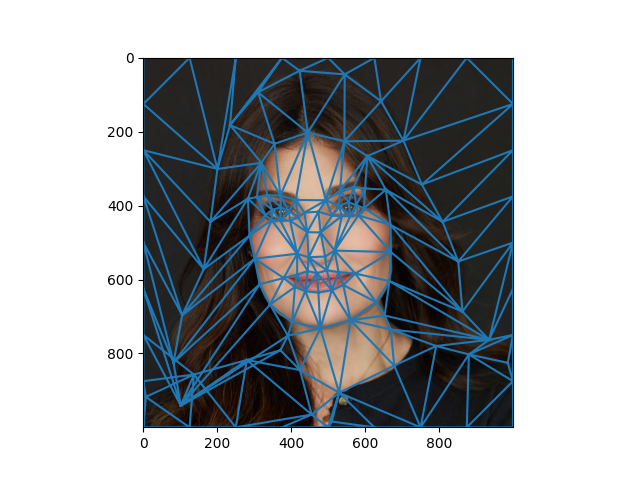
\includegraphics[width=\textwidth]{../visuals/average_idina_menzel_mesh.png}
    \end{subfigure}
    \begin{subfigure}{0.32\textwidth}
        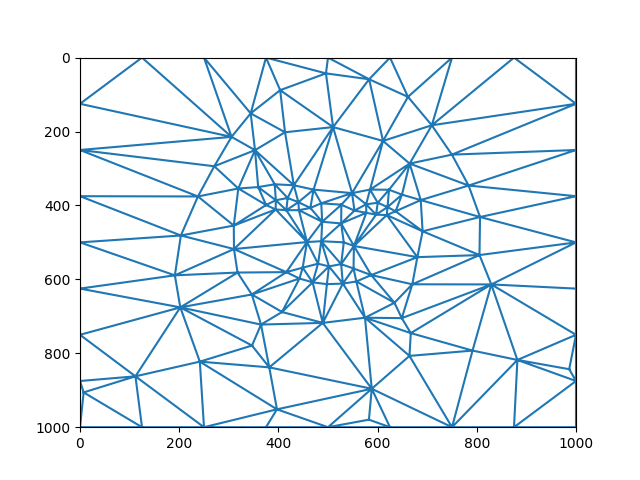
\includegraphics[width=\textwidth]{../visuals/average_mesh.png}
    \end{subfigure}
    \begin{subfigure}{0.32\textwidth}
        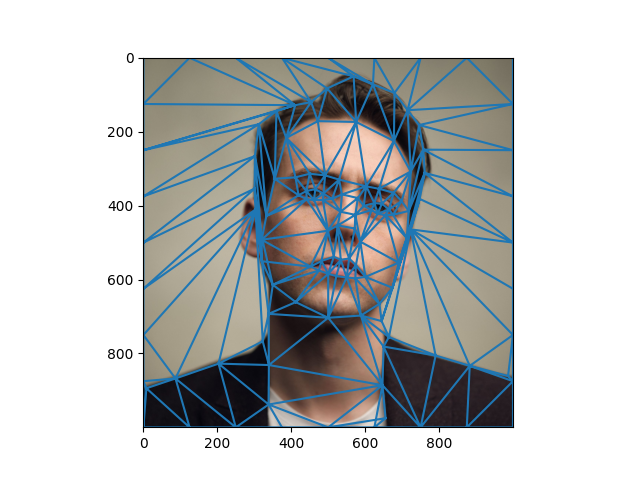
\includegraphics[width=\textwidth]{../visuals/average_jamie_muscato_mesh.png}
    \end{subfigure}
    \caption{The average mesh (middle) is triangulated through Delaunay triangulation, which is then mapped to the original points corresponding to the two faces. This allows for features such as the hair to be mapped one to one. We add points around the border to ensure the points are in a convex hull.}
\end{figure}

Once we have this triangulation, we need to map each simplex to another in a linear map. As this is a affine linear transformation between 2 dimensional shapes, we need a 3 dimensional matrix. We solve this by treating the 2D vectors to each corner of a triangle as 3D vectors with $z = 1$. This makes the vectors always linearly independent, allowing for a change of basis between the corners of one triangle to another triangle. In other words, our transformation between two matrices can be represented by the following matrix:
\[
    \begin{pmatrix}
        x_1' & x_2' & x_3' \\
        y_1' & y_2' & y_3' \\
        1 & 1 & 1
    \end{pmatrix}
    \begin{pmatrix}
        x_1 & x_2 & x_3 \\
        y_1 & y_2 & y_3 \\
        1 & 1 & 1
    \end{pmatrix}^{-1}.
\] 
Once we calculate which pixel is in which simplex (conversion to barycentric coordinates), for each frame, we can sample the color at the pixel after the linear map. However, we have a problem: the transform is continuous, but our images are made of discrete pixels.
\begin{figure}[H]
    \centering
    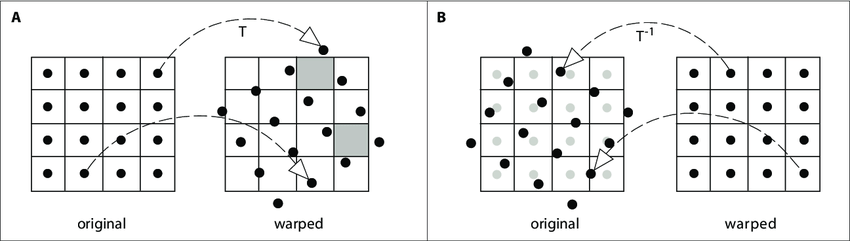
\includegraphics[width=0.7\textwidth]{../slides/public/imgs/sampling.png}
    \caption{Inverse vs Forward color sampling}
\end{figure}
We deal with this issue through inverse sampling. If transform from our source image to the frame, the resulting pixels can be spread apart due to the transformation, attentionally leaving massive gaps that are not colored. By inverting the transformation and determining the color of each pixel in the frame by mapping the matrix backwards, we can ensure that each pixel of our frame is colored. If the transformation lands between pixels, we use bilinear interpolation (weighted average of nearest 4 pixels) to choose the color. We sample the source and destination images weighted linearly through our translation, approximating a cross-fade.

Now that we have our interpolated images, we could extend this to only interpolate meshes instead of images. We implement this by only sampling our colors from the source image, resulting in our starting frame looking like our original image, but the image being slowly morphed into the destination mesh in any shape we want. We show two examples of this. The first is the creation of realistic caricatures by morphing the face mesh into the mesh of an existing caricature. The second application is simple animation, where we cause a flower to rotate and shrivel up simply by defining its initial and final mesh shapes.

\section*{Results}

\newcommand{\pad}[1]{0\ifnum#1<10 0\fi#1}

\begin{figure}[H]
    \foreach \i in {0,0,3,...,38,39,39} {
        \begin{subfigure}{0.125\textwidth}
            \includegraphics[width=\textwidth]{../frames/broadway/\pad{\i}.png}
        \end{subfigure}
        \hspace{-10pt}
    }
    \caption{Image morphing between Idina Menzel (Actor, Elphaba from \textit{Wicked}) and Jamie Muscato (Actor, JD from \textit{Heathers: The Musical}). Both meshes contain 94 points and results in 215 triangles. Images are both $1000 \times 1000$ pixels large. Each frame takes 15 seconds to generate.}
\end{figure}

\begin{figure}[H]
    \foreach \i in {0,0,3,...,38,39,39} {
        \begin{subfigure}{0.125\textwidth}
            \includegraphics[width=\textwidth]{../frames/brady/bradenberg_\pad{\i}.png}
        \end{subfigure}
        \hspace{-10pt}
    }
    \caption{Image morphing between Brady Bhalla (Student in CS 166) and Jesse Eisenberg (Actor, Brady's Doppelg\"anger). Both meshes contain 61 points, and images are both $500\times 500$ pixels large.}
\end{figure}

\begin{figure}[H]
    \centering
    \newcommand{\bleps}[1]{
        \foreach \i in {0,4,...,29} {
            \begin{subfigure}{0.125\textwidth}
                \includegraphics[width=\textwidth]{../frames/blep/#1_\pad{\i}.png}
            \end{subfigure}
            \hspace{-10pt}
        }
    }
    \bleps{blep12}
    \bleps{blep23}
    \bleps{blep34}
    \bleps{blep45}
    \bleps{blep51}

    \caption{Image morphing between images of 5 cats. The meshes were made by selecting a total 38 points around each of the cats' face, eyes, and tongue, resulting in a simple triangulation.}
\end{figure}

\begin{figure}[H]
    \centering
    \foreach \i in {0,6,...,39,39} {
        \begin{subfigure}{0.125\textwidth}
            \includegraphics[width=\textwidth]{../frames/flower/flower_rot_\pad{\i}.png}
        \end{subfigure}
        \hspace{-10pt}
    }
    \foreach \i in {0,6,...,39,39} {
        \begin{subfigure}{0.125\textwidth}
            \includegraphics[width=\textwidth]{../frames/flower/flower_close_\pad{\i}.png}
        \end{subfigure}
        \hspace{-10pt}
    }

    \caption{This time, color sampling is only done backwards to test the transitions of meshes between different images rather than interpolating between two images themselves. The flower has a simple mesh of 20 points rotated in the first row, then shrunk in the second row. This effectively creates an animation where we can warp the image as we wish in an intuitive manner.}
\end{figure}

\begin{figure}[H]
    \centering
    \begin{subfigure}{0.3\textwidth}
        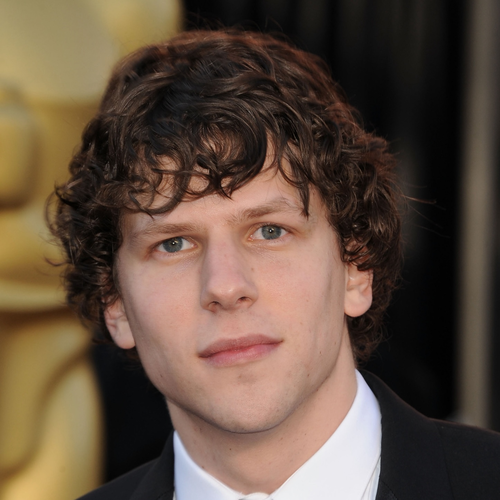
\includegraphics[width=\textwidth]{../input/jesse_eisenberg.png}
    \end{subfigure}
    \begin{subfigure}{0.3\textwidth}
        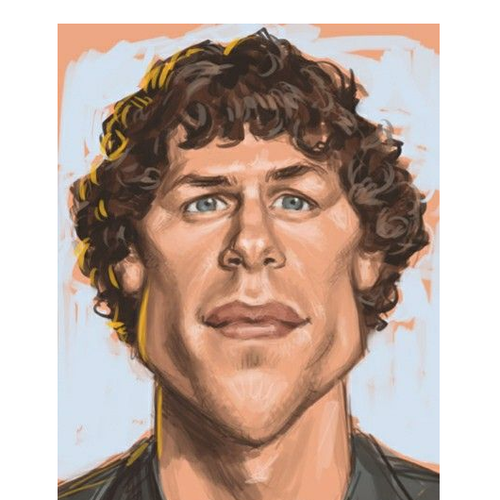
\includegraphics[width=\textwidth]{../input/caricuture.png}
    \end{subfigure}
    \begin{subfigure}{0.3\textwidth}
        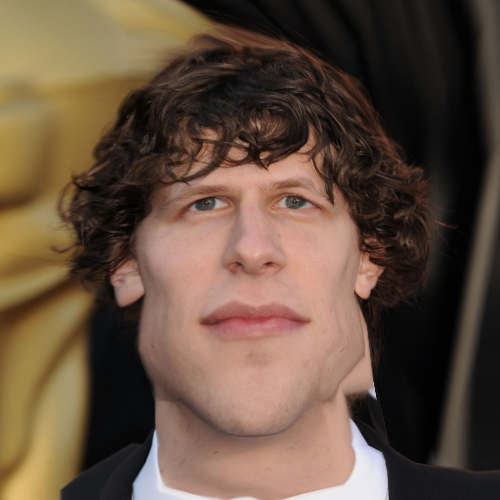
\includegraphics[width=\textwidth]{../frames/caricuture/caricuture_eisenberg_019.png}
    \end{subfigure}

    \caption{Morphing of meshes can also be used for just its final frame. By translating the mesh of Jesse Eisenberg's face into this caricature of Jesse Eisenberg, we can create a scary but realistic caricature of the actor. The mesh around both images are fairly simple, leading to a somewhat blocky look.}
\end{figure}

\section*{Challenges and Future Extensions}

Our algorithm is simple, which makes it very performant. The main purpose of this is to simplify the process of making meshes, but manually selecting points can still cause unexpected issues. For example in \textit{Figure 7}, we can see the right side of Jesse Eisenberg's face seems to be stretch out a bit because the triangulation decided the neck that was too close to the border was in fact part of the border. Although this can be mitigated by selecting better points for the mesh as well as extending the points in the border beyond the frame of the image, this can be a time consuming process.

One solution could be to introduce an algorithm that can recognize key features that correlate between two images to generate these points for us. For example, we could use a convolutional neural network trained on faces to highlight contours of the face and specific features, automating everything.

Although our algorithm works between images of different dimensions, it still scales linearly with the pixel count of the image as well as linearly the number of simplexes in our resulting mesh. This can result in possible slow downs for larger images. However, we propose that more complex algorithms such as Beier-Neely are a better fit for such projects.

It was challenging to debug many of the issues arising through the project, as there was no metric we could use to define what the ``correct'' results looked like, but everything worked out in the end. Overall, the project was interesting and gave some fun results.

\section*{Appendix: Code, Images, Meshes}

All code, input images, and generated meshes / images / gifs are stored in a Github repository: \href{https://github.com/ericlovesmath/image-morphing/tree/main}{https://github.com/ericlovesmath/image-morphing/tree/main}

\end{document}
